\begingroup
\renewcommand{\arraystretch}{1.45}
\fancyhead[L]{}
\fancyhead[C]{\small The Wonderful Pentagram}
\par\medskip\Needspace{5\baselineskip}\pdfbookmark[1]{Art. 2}{pentagramma-art-2}\centerline{[2.]}\nobreak\smallskip
The plane pentagon obtained by the central projection of that spherical pentagon onto an arbitrary plane has the property that the normals drawn from the individual vertices to the opposite side meet at one point (the viewpoint). At the same time, the products of the two parts into which that common intersection divides each normal are equal for all of them.

\providecommand{\EqOverGt}{\mathrel{\substack{=\\>}}}

\Needspace{30\baselineskip}
\SourceLeaf{492}

\begin{center}
\resizebox{.60\linewidth}{!}{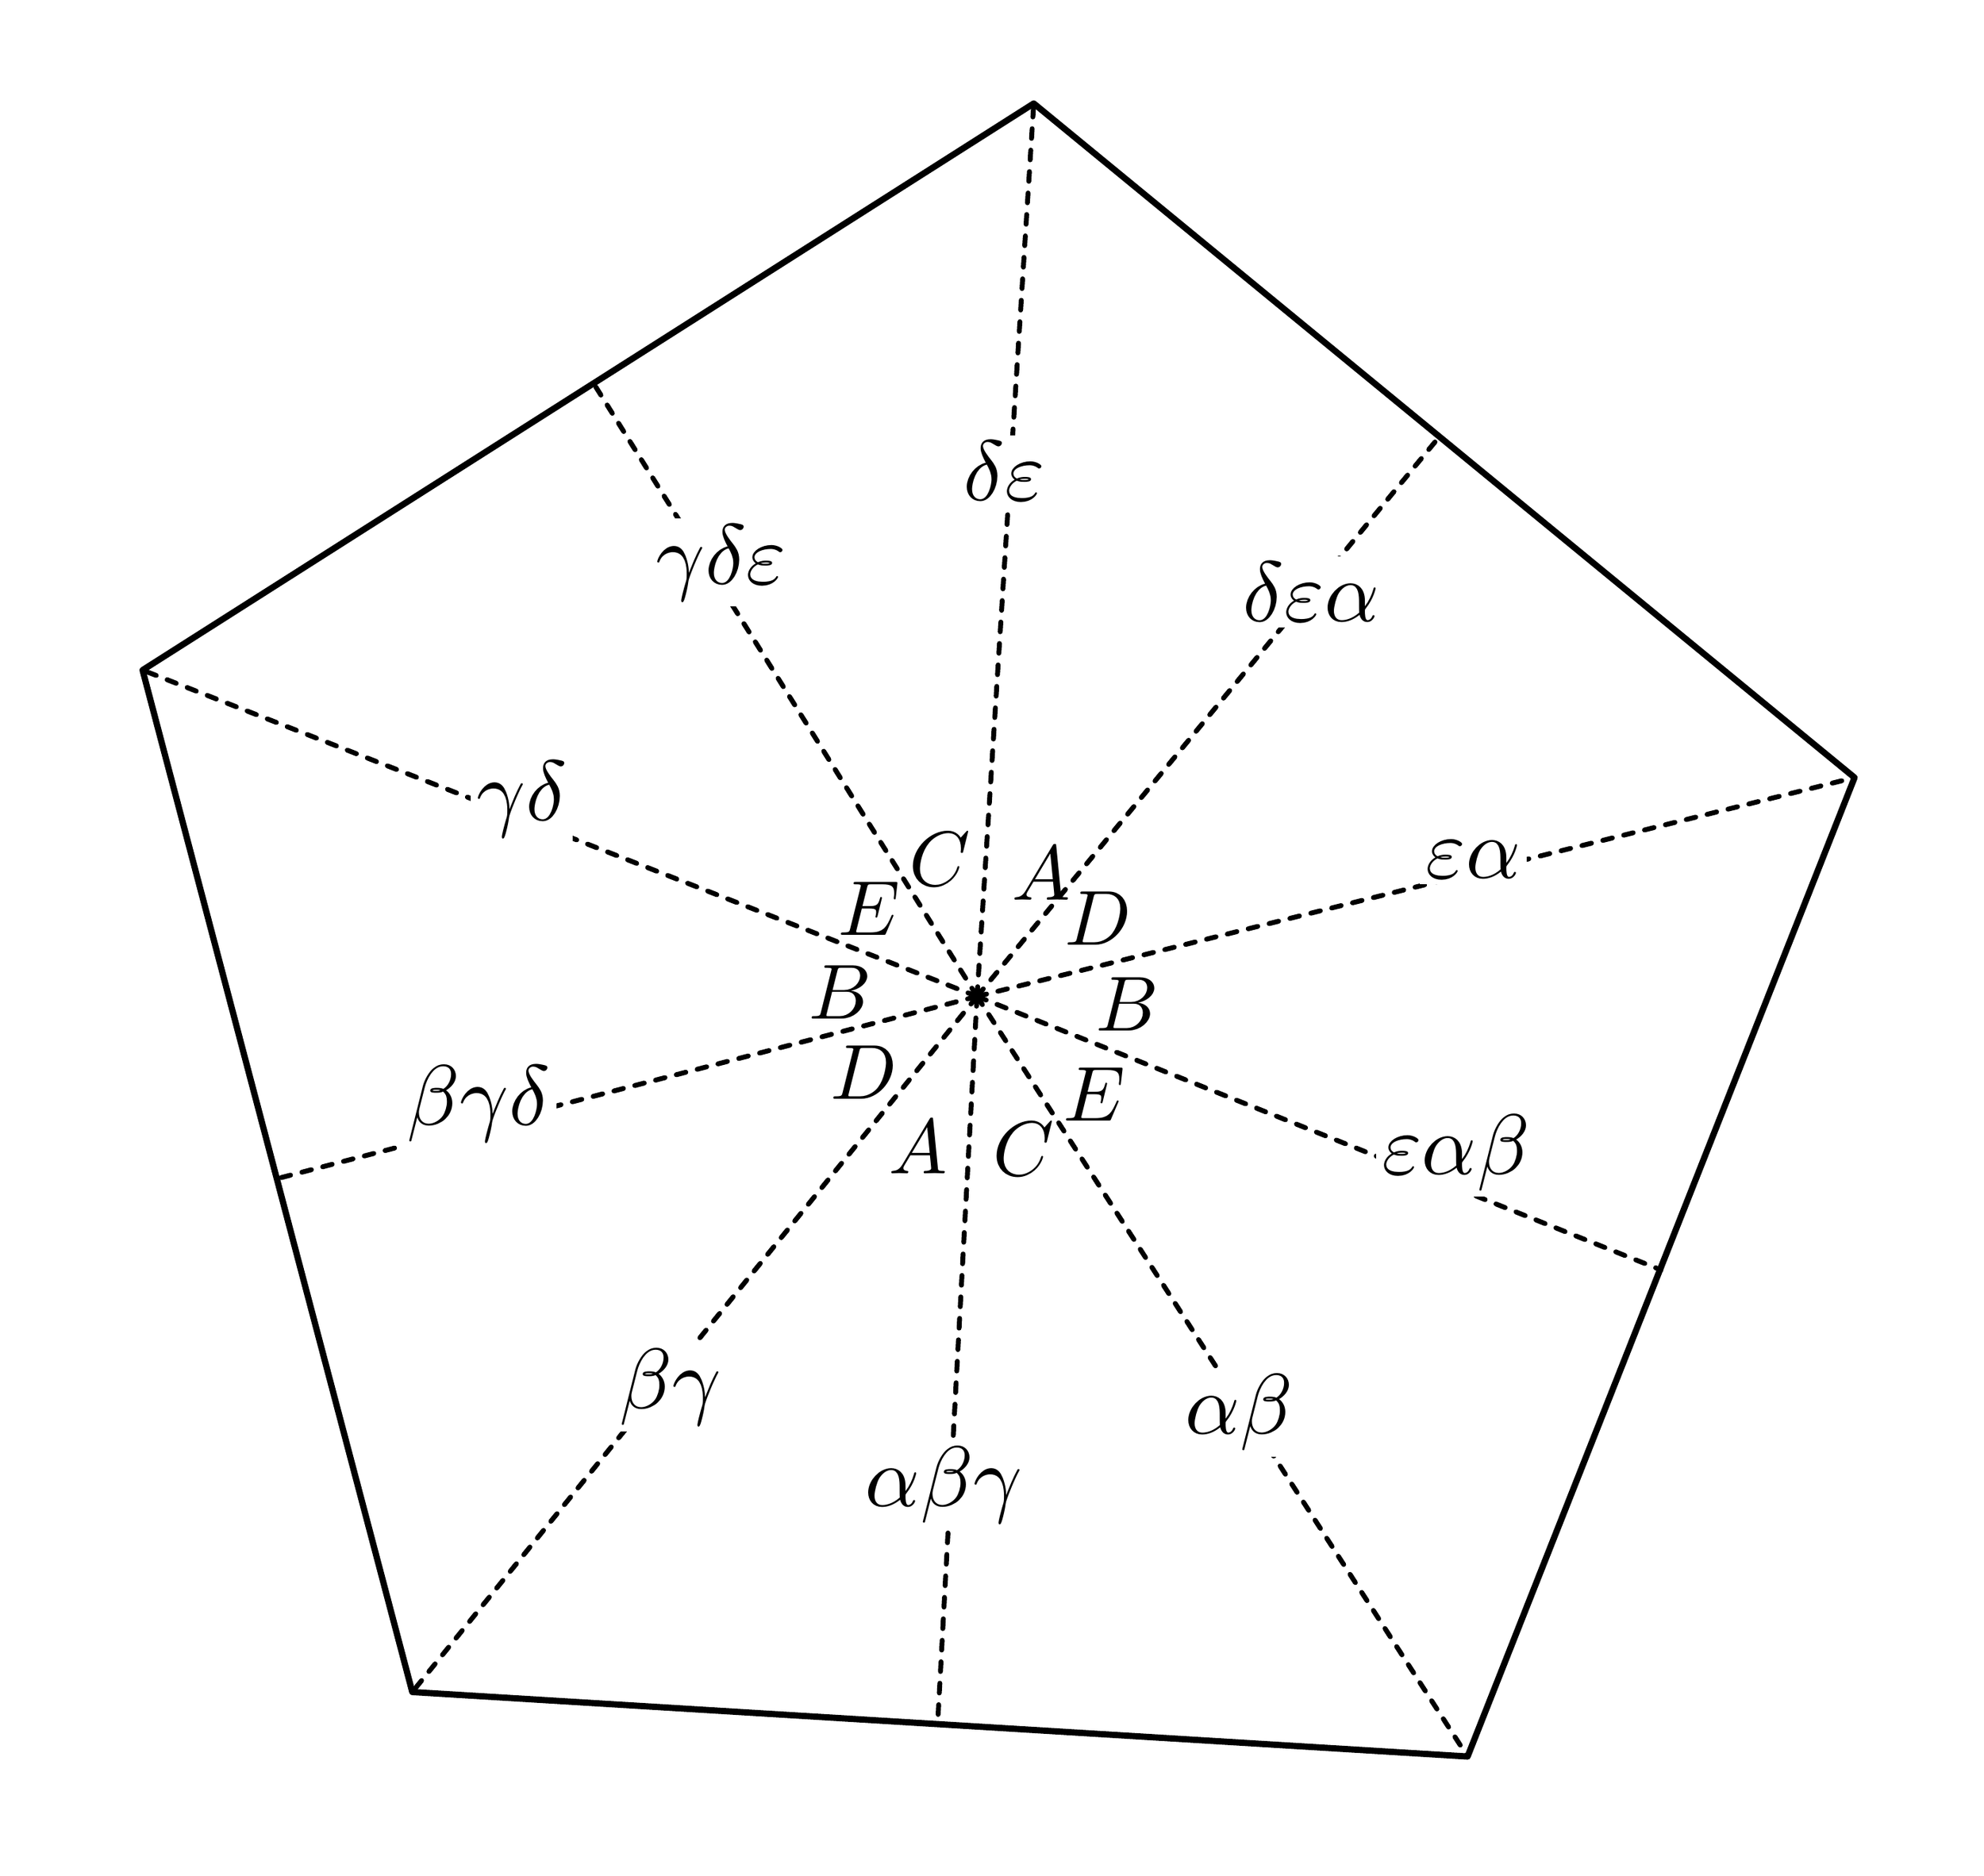
\begin{tikzpicture}[x=1bp,y=-1bp,line cap=round,line join=round]
\path[use as bounding box] (0,0) rectangle (995,940);
\begin{pgfinterruptboundingbox}
\draw[line width=3.2bp] (63,333) -- (519,43) -- (939,388) -- (741,889) -- (201,856) -- cycle;
\draw[line width=2.5bp,dash pattern=on 5bp off 6bp] (490,500) -- (293,185);
\draw[line width=2.5bp,dash pattern=on 5bp off 6bp] (490,500) -- (519,43);
\draw[line width=2.5bp,dash pattern=on 5bp off 6bp] (490,500) -- (727,213);
\draw[line width=2.5bp,dash pattern=on 5bp off 6bp] (490,500) -- (939,388);
\draw[line width=2.5bp,dash pattern=on 5bp off 6bp] (490,500) -- (840,640);
\draw[line width=2.5bp,dash pattern=on 5bp off 6bp] (490,500) -- (741,889);
\draw[line width=2.5bp,dash pattern=on 5bp off 6bp] (490,500) -- (470,869);
\draw[line width=2.5bp,dash pattern=on 5bp off 6bp] (490,500) -- (201,856);
\draw[line width=2.5bp,dash pattern=on 5bp off 6bp] (490,500) -- (129,594);
\draw[line width=2.5bp,dash pattern=on 5bp off 6bp] (490,500) -- (63,333);
\node[fill=white,inner sep=3bp,outer sep=0pt,rotate=0] at (504,231) {\scalebox{4.4}{\ensuremath{\delta\varepsilon}}};
\node[fill=white,inner sep=3bp,outer sep=0pt,rotate=0] at (661,293) {\scalebox{4.4}{\ensuremath{\delta\varepsilon\alpha}}};
\node[fill=white,inner sep=3bp,outer sep=0pt,rotate=0] at (744,430) {\scalebox{4.4}{\ensuremath{\varepsilon\alpha}}};
\node[fill=white,inner sep=3bp,outer sep=0pt,rotate=0] at (735,580) {\scalebox{4.4}{\ensuremath{\varepsilon\alpha\beta}}};
\node[fill=white,inner sep=3bp,outer sep=0pt,rotate=0] at (624,713) {\scalebox{4.4}{\ensuremath{\alpha\beta}}};
\node[fill=white,inner sep=3bp,outer sep=0pt,rotate=0] at (473,750) {\scalebox{4.4}{\ensuremath{\alpha\beta\gamma}}};
\node[fill=white,inner sep=3bp,outer sep=0pt,rotate=0] at (333,700) {\scalebox{4.4}{\ensuremath{\beta\gamma}}};
\node[fill=white,inner sep=3bp,outer sep=0pt,rotate=0] at (235,555) {\scalebox{4.4}{\ensuremath{\beta\gamma\delta}}};
\node[fill=white,inner sep=3bp,outer sep=0pt,rotate=0] at (257,399) {\scalebox{4.4}{\ensuremath{\gamma\delta}}};
\node[fill=white,inner sep=3bp,outer sep=0pt,rotate=0] at (359,278) {\scalebox{4.4}{\ensuremath{\gamma\delta\varepsilon}}};
\node[inner sep=0pt,outer sep=0pt,rotate=0] at (471,430) {\scalebox{4.0}{\ensuremath{C}}};
\node[inner sep=0pt,outer sep=0pt,rotate=0] at (523,437) {\scalebox{4.0}{\ensuremath{A}}};
\node[inner sep=0pt,outer sep=0pt,rotate=0] at (552,460) {\scalebox{4.0}{\ensuremath{D}}};
\node[inner sep=0pt,outer sep=0pt,rotate=0] at (567,504) {\scalebox{4.0}{\ensuremath{B}}};
\node[inner sep=0pt,outer sep=0pt,rotate=0] at (550,550) {\scalebox{4.0}{\ensuremath{E}}};
\node[inner sep=0pt,outer sep=0pt,rotate=0] at (514,578) {\scalebox{4.0}{\ensuremath{C}}};
\node[inner sep=0pt,outer sep=0pt,rotate=0] at (460,577) {\scalebox{4.0}{\ensuremath{A}}};
\node[inner sep=0pt,outer sep=0pt,rotate=0] at (432,539) {\scalebox{4.0}{\ensuremath{D}}};
\node[inner sep=0pt,outer sep=0pt,rotate=0] at (420,498) {\scalebox{4.0}{\ensuremath{B}}};
\node[inner sep=0pt,outer sep=0pt,rotate=0] at (435,455) {\scalebox{4.0}{\ensuremath{E}}};
\end{pgfinterruptboundingbox}
\end{tikzpicture}
}
\end{center}
\[
\begin{gathered}\cos A=\alpha,\quad \cos B=\beta,\quad \cos C=\gamma,\\[9pt]\quad{}\quad \cos D=\delta,\quad \cos E=\varepsilon\end{gathered}
\]

To obtain the vertices expressed by complex integers, let $p,p',p'',p''',p''''$ be five complex integers, namely
\[
p=a+bi,\quad p'=a'+b'i,\quad\text{etc.}
\]
Set
\[
a'a'''+b'b'''=(1,3),\quad a''a''''+b''b''''=(2,4)\quad\text{etc.}
\]

\Needspace{10\baselineskip}
and take for the vertices
\par\nopagebreak% portrait-table start
\begingroup\small\setlength{\arraycolsep}{2pt}\[
\resizebox{.98\linewidth}{!}{$\displaystyle \begin{array}{rccccc} & (1,3)(2,4)p, & (2,4)(3,0)p', & (3,0)(4,1)p'', & (4,1)(0,2)p''', & (0,2)(1,3)p''''\\[9pt] = & q, & q', & q'', & q''', & q'''' \end{array}$}
\]\endgroup\par% portrait-table end

\Needspace{14\baselineskip}
thus
\[
\begin{gathered} q=(a'a'''+b'b''')(a''a''''+b''b'''')a \\[9pt]\quad{}+(a'a'''+b'b''')(a''a''''+b''b'''')bi\\[9pt] \qquad\text{and so on} \end{gathered}
\]
Then
\[
\begin{gathered} q'-q=(ba'-ab')(2,4)(b'''-a'''i)\\[9pt]\quad{}=-(ba'-ab')(2,4)p'''i\\[9pt] \qquad\text{and so on} \end{gathered}
\]




\Needspace{24\baselineskip}
\SourceLeaf{493}

The intersection of $qq'$ with $oq'''$ has the complex number $=$
\[
Q'''=\frac{(1,3)(2,4)(3,0)}{a'''a'''+b'''b'''}p''' \quad\text{etc.}
\]
The product mentioned above becomes
\[
\begin{gathered}  =-(0,2)(1,3)(2,4)(3,0)(4,1)\\[9pt] Q'''-q=\frac{(1,3)(2,4)(ba'''-ab''')}{a'''a'''+b'''b'''} (b'''-a'''i)\\[9pt] q'-Q'''=\frac{(2,4)(3,0)(a'b'''-b'a''')}{a'''a'''+b'''b'''} (b'''-a'''i) \end{gathered}
\]
\clearpage
\endgroup
